\documentclass{article}
\usepackage{geometry}
\usepackage{graphicx}
\usepackage{amsmath}
\usepackage{algorithm}
\usepackage{algpseudocode}
\usepackage{dsfont}
\usepackage{amssymb}
\usepackage{multicol}
\usepackage{wrapfig}
\geometry{
a4paper,
right=10mm,
left=10mm,
top=10mm,
bottom=10mm,	
}

\begin{document}

\pagenumbering{gobble}

\begin{center}
\textbf{\Large HOMEWORK 2 : CS771} \\
\textit{\large Jayant Agrawal}         14282
\end{center}
\section{Problem 1}
\begin{figure}[h!]
\centering
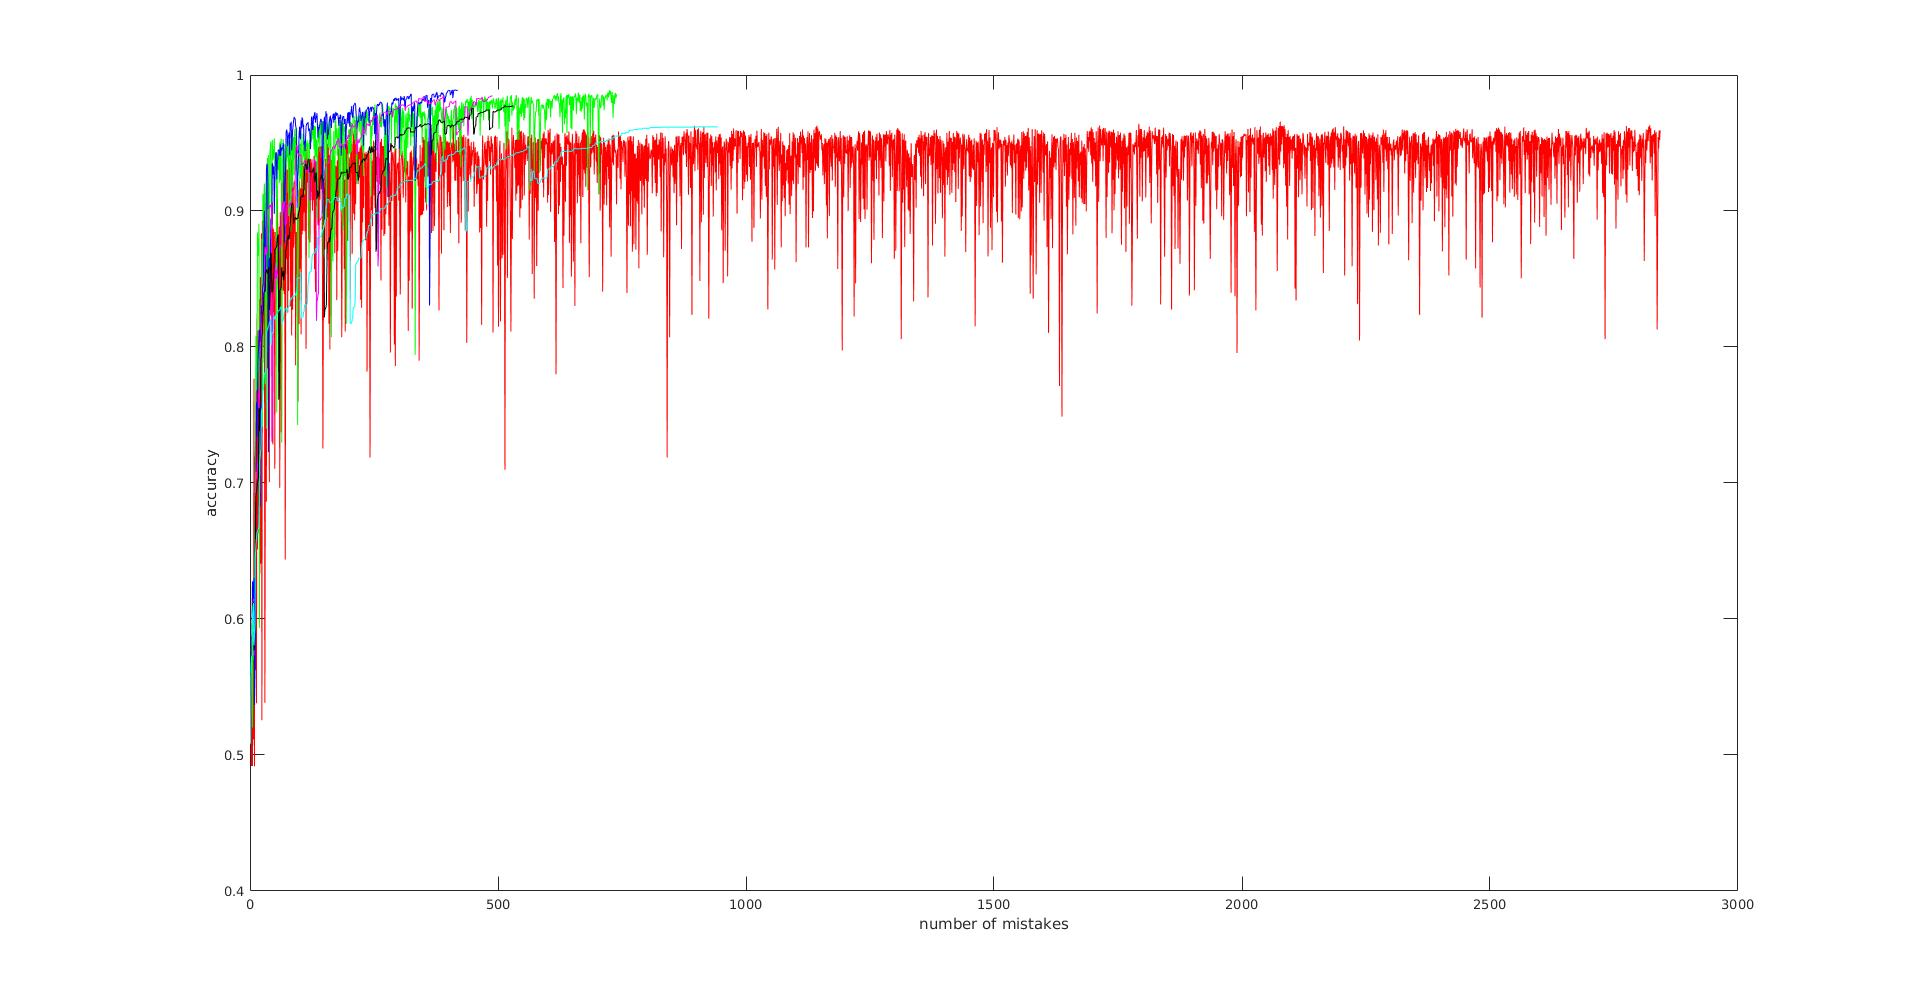
\includegraphics[width=0.8\columnwidth]{plot_acc.jpg}
\caption{Classification Accuracy: Simple(Red) and Averaged(Green)}
\label{acc}
\end{figure}

\begin{itemize}
\item The curve with Rupert-Polyak Averaging has higher accuracy than the the one without averaging.
\item The updates without averaging depend too much on the latest example, and does not capture the training set, therefore weigths learned are not so optimal.
\item The curves attain near optimal accuracy quickly and then the accuracy remains close to the optimal accuracy for both the cases.
\item However, for non-averaged version, since the lates update is influenced heavily by the latest example, the accuracy fluctuations are high.
\item Updating with Rupert-Polyak Averging significantly reduces the updates' dependence on the latest examples and captures information from a larger subset of training data at a time. It thus removes all the fluctuations from the accuracy curve.
\item The model without averaging is penalized heavily by the outliers at each update, whereas the impact of outliers is almost removed in averaged version.
\end{itemize}

\section{Problem 2}
\subsection{Fig 1}
\begin{figure}[h!]
\begin{center}
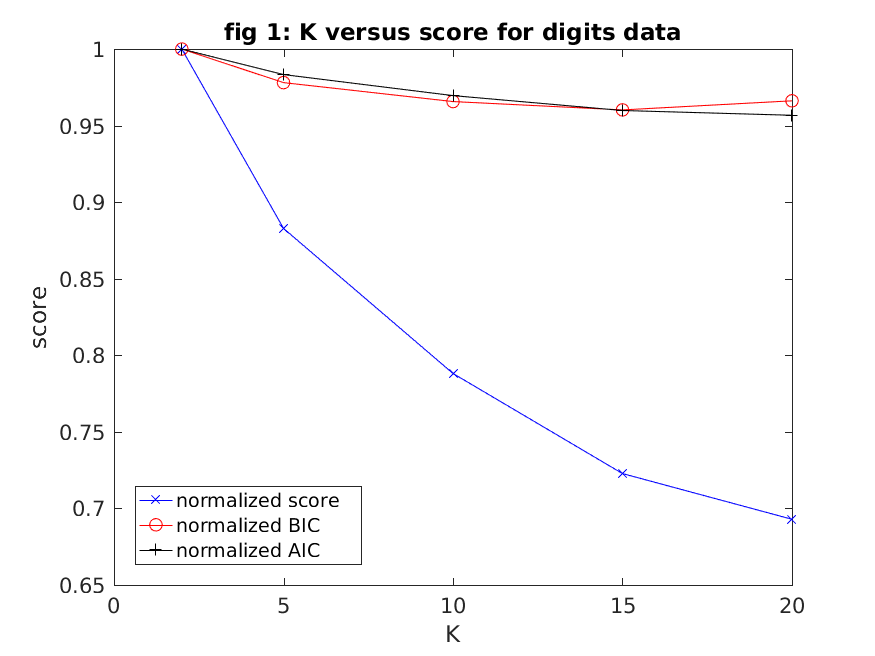
\includegraphics[width=0.5\columnwidth]{RunResults2/1.png}
\label{1}
\end{center}
\end{figure}

\subsubsection{Trends}
\begin{itemize}
\item \emph{The score decreases as K increases.} This had to be the case, since now the sum of distances from data points to their nearest cluster centers decreases, simply because of increase in the number of centers.
\item \emph{The rate of decrease in Score decreases with increase in K.}
\item \emph{BIC scores first decreases then increases.} After a certain point, the second term in BIC which is proportional to  K, starts weiging more than the score, thus BIC starts increasing. AIC will also show a similar behavior for larger K.
\end{itemize}

\subsubsection{Choice of K}
\begin{itemize}
\item \textbf{Score: } On the basis of Score, the choice can be made by looking at the \emph{"elbow-point"}. In this case the elbow point seems to be 15. If the graph is plotted for more values of K, the elbow point will be closer to 10 (digits).
\item \textbf{BIC: }BIC penalizes large values of K, as can be observed from the graph. The choice for K should be made such that BIC is minimum which for this case is 15. Again, plotting the graph with more values of K, would ensure the minima to be closer to 10.
\item \textbf{AIC: }Similar to BIC, AIC also penalizes large values of K. But since it does not contain the factor of $log(n)$, the effect would be seen a bit later. For this case, the choice of K using AIC is 20.
\end{itemize}

\subsection{Fig 2}
\begin{figure}[h!]
\begin{center}
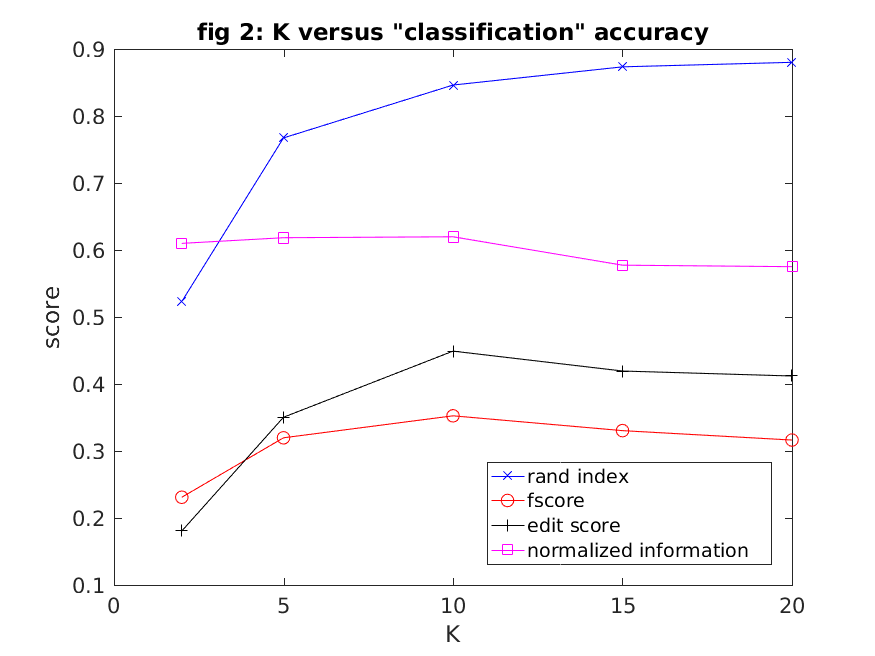
\includegraphics[width=.5\columnwidth]{RunResults2/2.png}
\label{2}
\end{center}
\end{figure}

\begin{itemize}
\item Since, we know the Gold Truth(K=10), and higher is better, the plot which gives maxima at K=10 should be a good choice. Hence "edit score" is the most reasonable choice.
\item The rand index increases sharply till 10, after which the rate of increase decreases.
\item The curve given by fscore also has a maxima at k=10 after which it saturates. 
\item Based on these observations, K=10 should be selected.
\end{itemize}

\subsection{Fig 3-5}
%\begin{left}

\begin{figure}[h!]
\begin{multicols}{3}
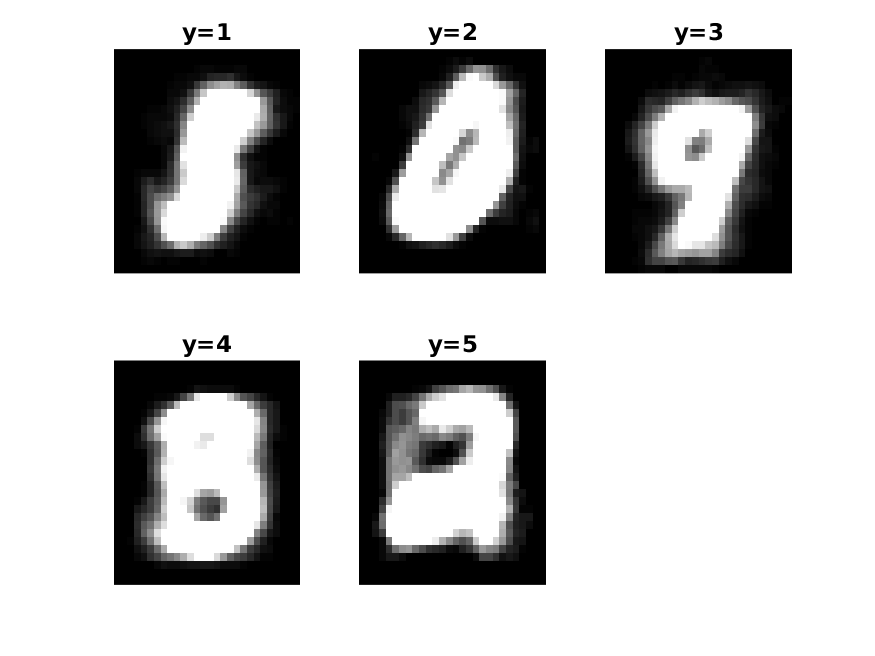
\includegraphics[width=1\columnwidth]{RunResults2/3.png}
\label{3}
%\caption{Fig 3}

%\end{left}
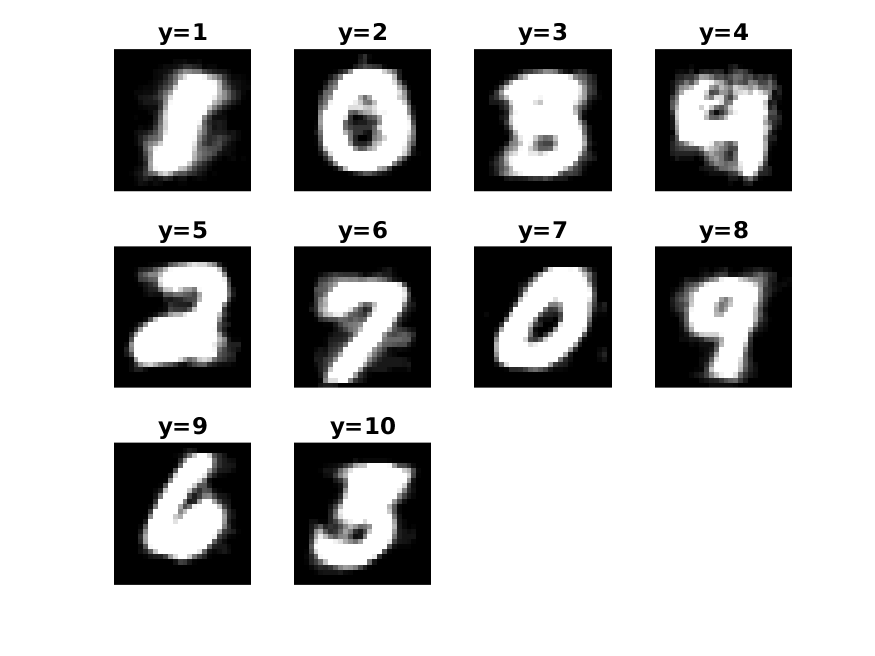
\includegraphics[width=1\columnwidth]{RunResults2/4.png}
\label{4}
%\caption{Fig 4}

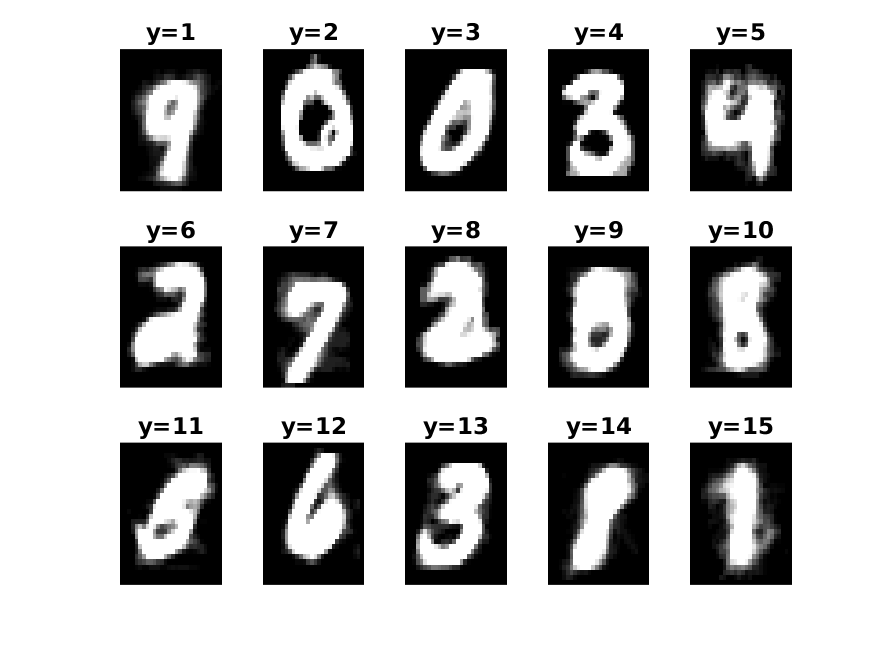
\includegraphics[width=1\columnwidth]{RunResults2/5.png}
\label{5}
%\caption{Fig 5}
\end{multicols}
\end{figure}

\subsubsection{Fig 3}
\emph{Recognisable: } 0,9,2   \hspace{2cm}   \emph{Missing: } 4,6,7 \hspace{2cm}    \emph{Merged: } (1,5), (3,8)

\subsubsection{Fig 4}
\emph{Recognisable: } 1,0,4,2,7,9,6,3 \hspace{2cm} \emph{Missing: } 5,8 \hspace{2cm} \emph{Merged: } (3,5), (3,8)

\subsubsection{Fig 5}
\emph{Recognisable: } 9,0,3,4,2,7,6,8,5,3,1 \hspace{2cm} \emph{Missing: }  None \hspace{2cm} \emph{Merged: } (5,6), (6,8)

\subsection{Fig 6}
\begin{figure}[h!]
\begin{center}
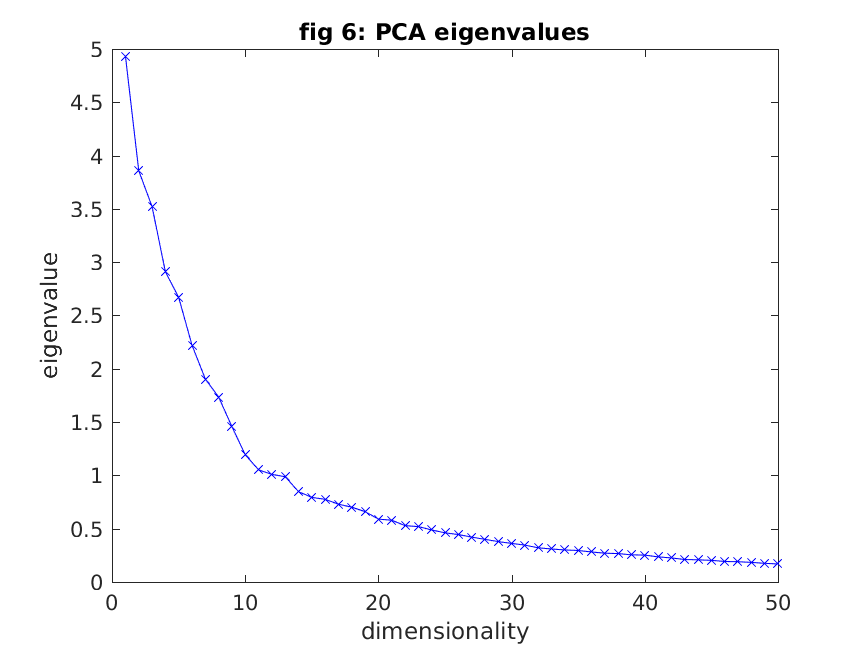
\includegraphics[width=1\columnwidth]{RunResults2/6.png}
\label{6}
\end{center}
\end{figure} 
The incentive for increasing the dimensionality starts to significanly decrease nearly after 10. The rate of decrease further decreases after \textbf{20} in this case.
\newpage
\subsection{ Fig 7}
\begin{figure}[h!]
\begin{center}
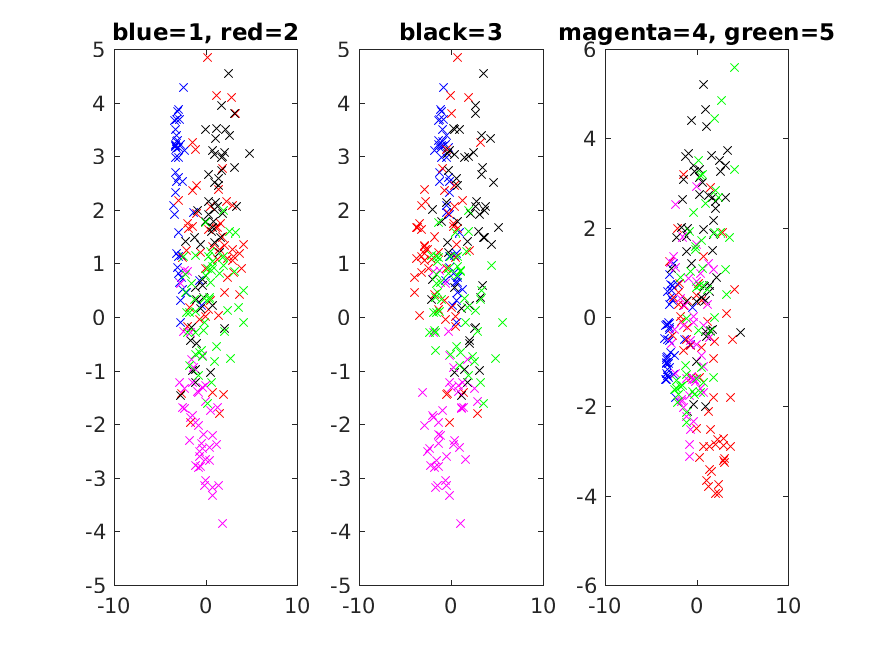
\includegraphics[width=0.5\columnwidth]{RunResults2/7.png}
\label{7}
\end{center}
\end{figure}

\begin{itemize}
\item The digits that are scattered more are more confusable.
\item The digits in the order of their confusability are: 3 > 5 > 2 > 1 > 4.
\item Since 3 and 5 have similar structure, they are more confusable. This make sense because they are more scattered in the figure. 
\end{itemize}

\subsection{Fig 8-12}
\begin{figure}[h!]
\begin{multicols}{3}
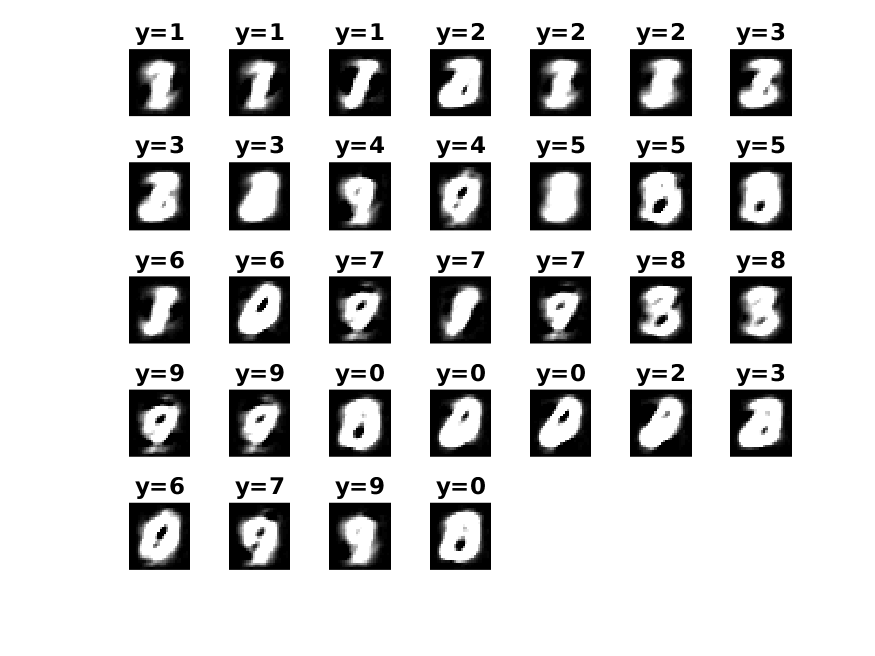
\includegraphics[width=1\columnwidth]{RunResults2/8.png}
\label{8}

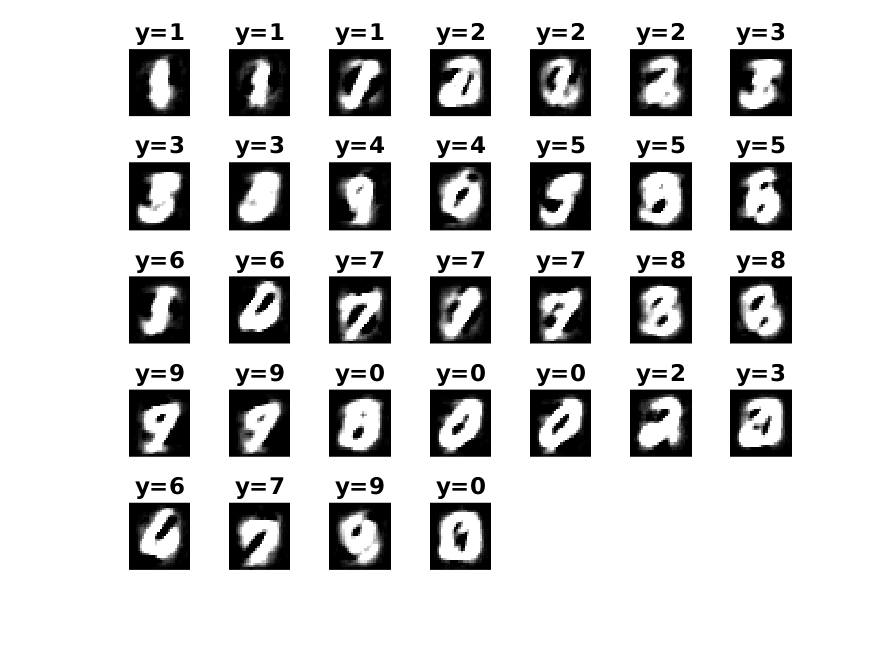
\includegraphics[width=1\columnwidth]{RunResults2/9.png}
\label{9}

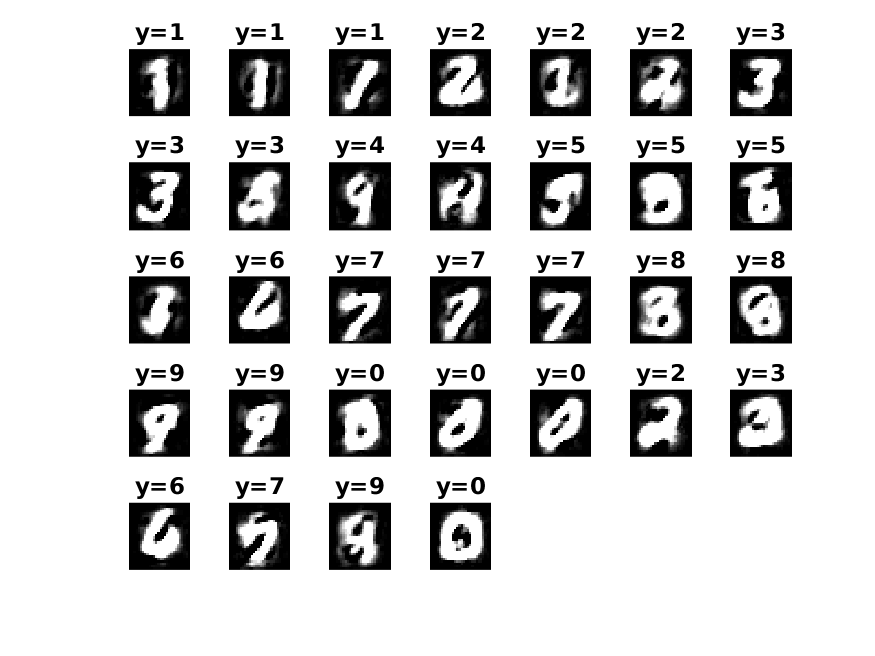
\includegraphics[width=1\columnwidth]{RunResults2/10.png}
\label{10}
\end{multicols}
\centering
\begin{multicols}{2}
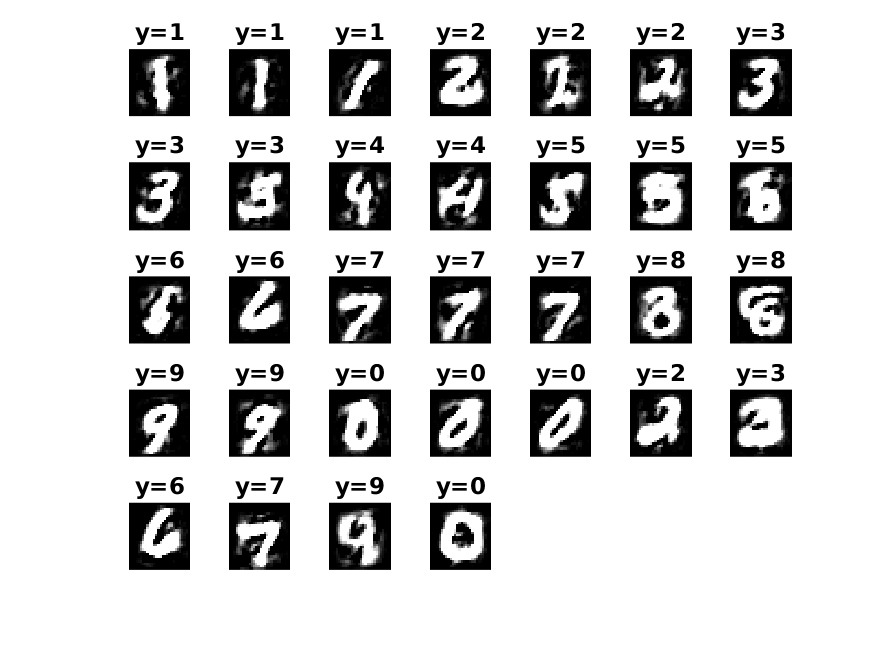
\includegraphics[width=0.65\columnwidth]{RunResults2/11.png}
\label{11}

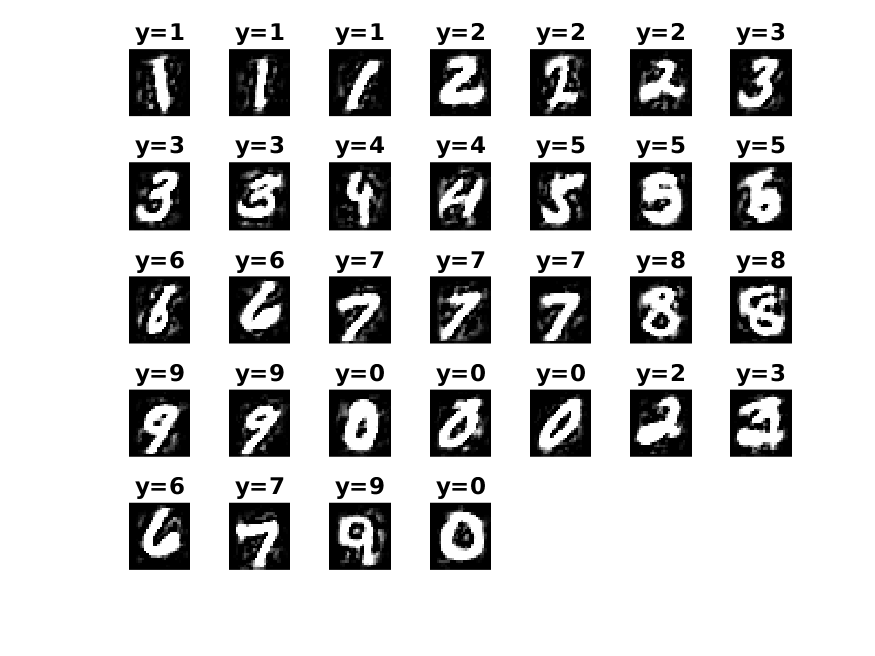
\includegraphics[width=0.65\columnwidth]{RunResults2/12.png}
\label{12}

\end{multicols}
\end{figure}
Some digits become recognisable at 12 dimensions. However, most digits are recognisable at \textbf{20} dimensions. This agrees with \ref{6}, as the "rate of decrease" decreases substantially after 20 dimensions in the graph. \\
\newpage
\subsection{Fig 13}
\begin{figure}[h!]
\begin{center}
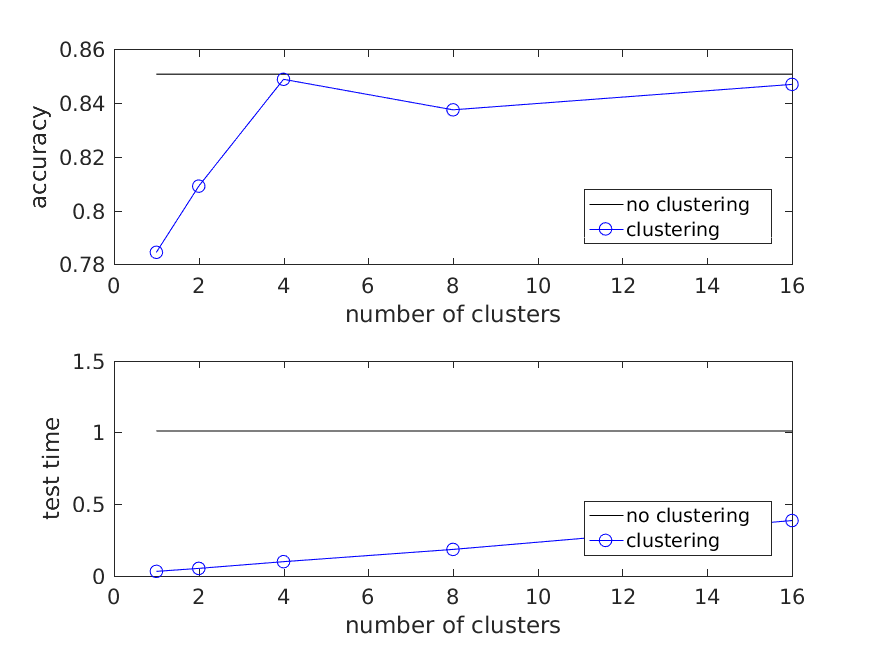
\includegraphics[width=0.5\columnwidth]{RunResults2/13.png}
\label{13}
\end{center}
\end{figure}
At K=8 accuracy is greater than 1-NN. At test time accuracy changes with K. It is useful in practice.


\subsection{Fig 14}
\begin{figure}[h!]
\begin{center}
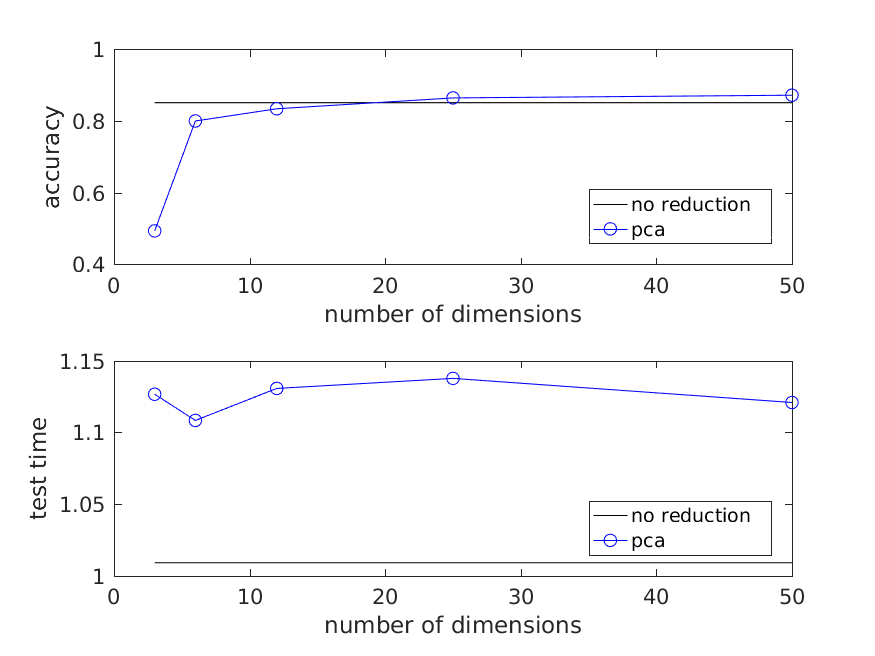
\includegraphics[width=0.5\columnwidth]{RunResults2/14.png}
\label{14}
\end{center}
\end{figure}
The accuracy increases with number of dimensions. The accuracy for PCA is greater than 1-NN after K=20. At test time, there is no particular relation with 1-NN. It can be used in practice since the accuracy is better than 1-NN.
\section{Problem 3}
As discussed in class, $y_n \in {0,1,2, ... K-1}$ and label probabilities are defined as:
$$p(y_n=k|x_n,W) = \frac{exp(w_k^\top x_n)}{\sum_{l=1}^{K}exp(w_l^\top x_N)} = \mu_{nk}$$
\\
Log Likelihood is given as:
\begin{equation*}
\begin{aligned}
log(\prod_{n=1}^N p(y_n|x_n,W)) &=  \sum_{n=1}^N log(\mu_{ny_n}) \\
&=  \sum_{n=1}^N log(\frac{exp(w_{y_n}^\top)x_n}{\sum_{l=1}^K exp(w_l^\top x_N)}) \\ 
&= \sum_{n=1}^N [w_{y_n}^\top x_n - log(\sum_{l=1}^K exp(w_l^\top x_N))] \\ 
\end{aligned}
\end{equation*}

Thus, Negative Log Likelihood is given by:
$$NLL(W) =  -\sum_{n=1}^N [w_{y_n}^\top x_n - log(\sum_{l=1}^K exp(w_l^\top x_n))]  $$

Now, taking the derivative w.r.t $w_k$ to get gradient $g_k$ :
\begin{equation*}
\begin{aligned}
g_k = \frac{\partial(NLL(W))}{\partial w_k} \\
\end{aligned}
\end{equation*}
Therefore $g_k$ is:
\begin{equation*}
\begin{aligned}
g_k &= \frac{\partial}{\partial w_k}(-\sum_{n=1}^N [w_{y_n}^\top x_n - log(\sum_{l=1}^K exp(w_l^\top x_n))]) \\ 
&= - \sum_{n=1}^N [\frac{\partial w_{y_n}^\top}{\partial w_k} - \frac{\sum_{l=1}^K (exp(w_l^\top x_n)\frac{\partial w_l^\top }{\partial w_k})}{\sum_{l=1}^K exp(w_l^\top x_n)}]x_n \\
&= - \sum_{n=1}^N [y_{nk} - \frac{exp(w_k^\top x_n)}{\sum_{l=1}^K exp(w_l^\top x_n)}]x_n \\
&= \sum_{n=1}^N [\mu_{nk} - y_{nk} ]x_n \\
\end{aligned}
\end{equation*}
where $y_{nk}=1$, when $y_n = k$, 0 otherwise. \\
Thus, the gradient based update rule, for $w_k$ is:
$$w_k^{t+1} = w_k^{t} - \eta \sum_{n=1}^N [\mu_{nk} - y_{nk} ]x_n$$
\section{Problem 4}

Let the set of points ${x_1,x_2,...x_N}$ and ${y_1,y_2,...y_n}$ be the sets X and Y respectively.\\ \\
\emph{Direction 1: If X and Y are linearly separable, then the convex hulls do not intersect.} \\

If the sets are linearly separable, there exists a pair $w \in \mathds{R}^n$, $b \in \mathds{R}$, such that :
$$w.x_i + b > 0 \forall x_i \in X$$
$$w.y_i + b < 0 \forall y_i \in Y$$

Assume that the convex hulls intersect, then there exists a point z, such that it can be written as:
$$z = \sum_n \alpha_n x_n = \sum_m \beta_m y_m$$
for some $\alpha$ and $\beta$. Now, consider, $\sum_n \alpha_n(w.x_i + b)$, this is clearly positve. Similarly, $\sum_m \beta_m(w.y_i + b)$ is clearly negative. But, both are same and equal to z. Thus, we get a contradiction.\\ \\
\emph{Direction 2: If the convex hulls do not intersect, then the sets are linearly separable.} \\

Let $CH_X$ and $CH_Y$ be the convex hulls of X and Y. Also, let $C = CH_X-CH_Y$ denote the set of points whose position vectors are given by x-y for some $x \in CH_X$ and $y \in CH_Y$. Since, the convex hulls do not intersect, C does not contain the origin.\\

Also, since $CH_X$ and $CH_Y$ are convex, thus C is also a convex set. Now, consider a point $z_1 \in C$, which is the nearest to origin. Assume that there exists a point $z$, such that $z.z_1 \leq 0$. Also, all the points lying on the line joining $z$ and $z_1$, belong to C (by Convexity). \\

Now, define $u= (z-z_1)/||z-z_1||^2 $, and the distance from the closest point on the line joining $z$ and $z_1$ and origin is $||z_1||^2 - (z_1.u)^2$, which is less than the distance of $z_1$ from origin. We thus get a contradiction. Thus, $z.z_1 > 0$ for all points z in C. Therefore, C is linearly separable from origin. Hence, $CH_X-CH_Y$ and X -Y are linearly separable from origin. This shows that X is linearly separable from Y. \\ \\
The above claims show that the set of xs and the set of ys are linearly separable if and only if the convex hulls do not intersect.
\end{document}


